\thispagestyle{thachthuctoanhocnone}
\pagestyle{thachthuctoanhoc}
\everymath{\color{thachthuctoanhoc}}
\graphicspath{{../thachthuctoanhoc/pic/}}
\begingroup
\AddToShipoutPicture*{\put(0,616){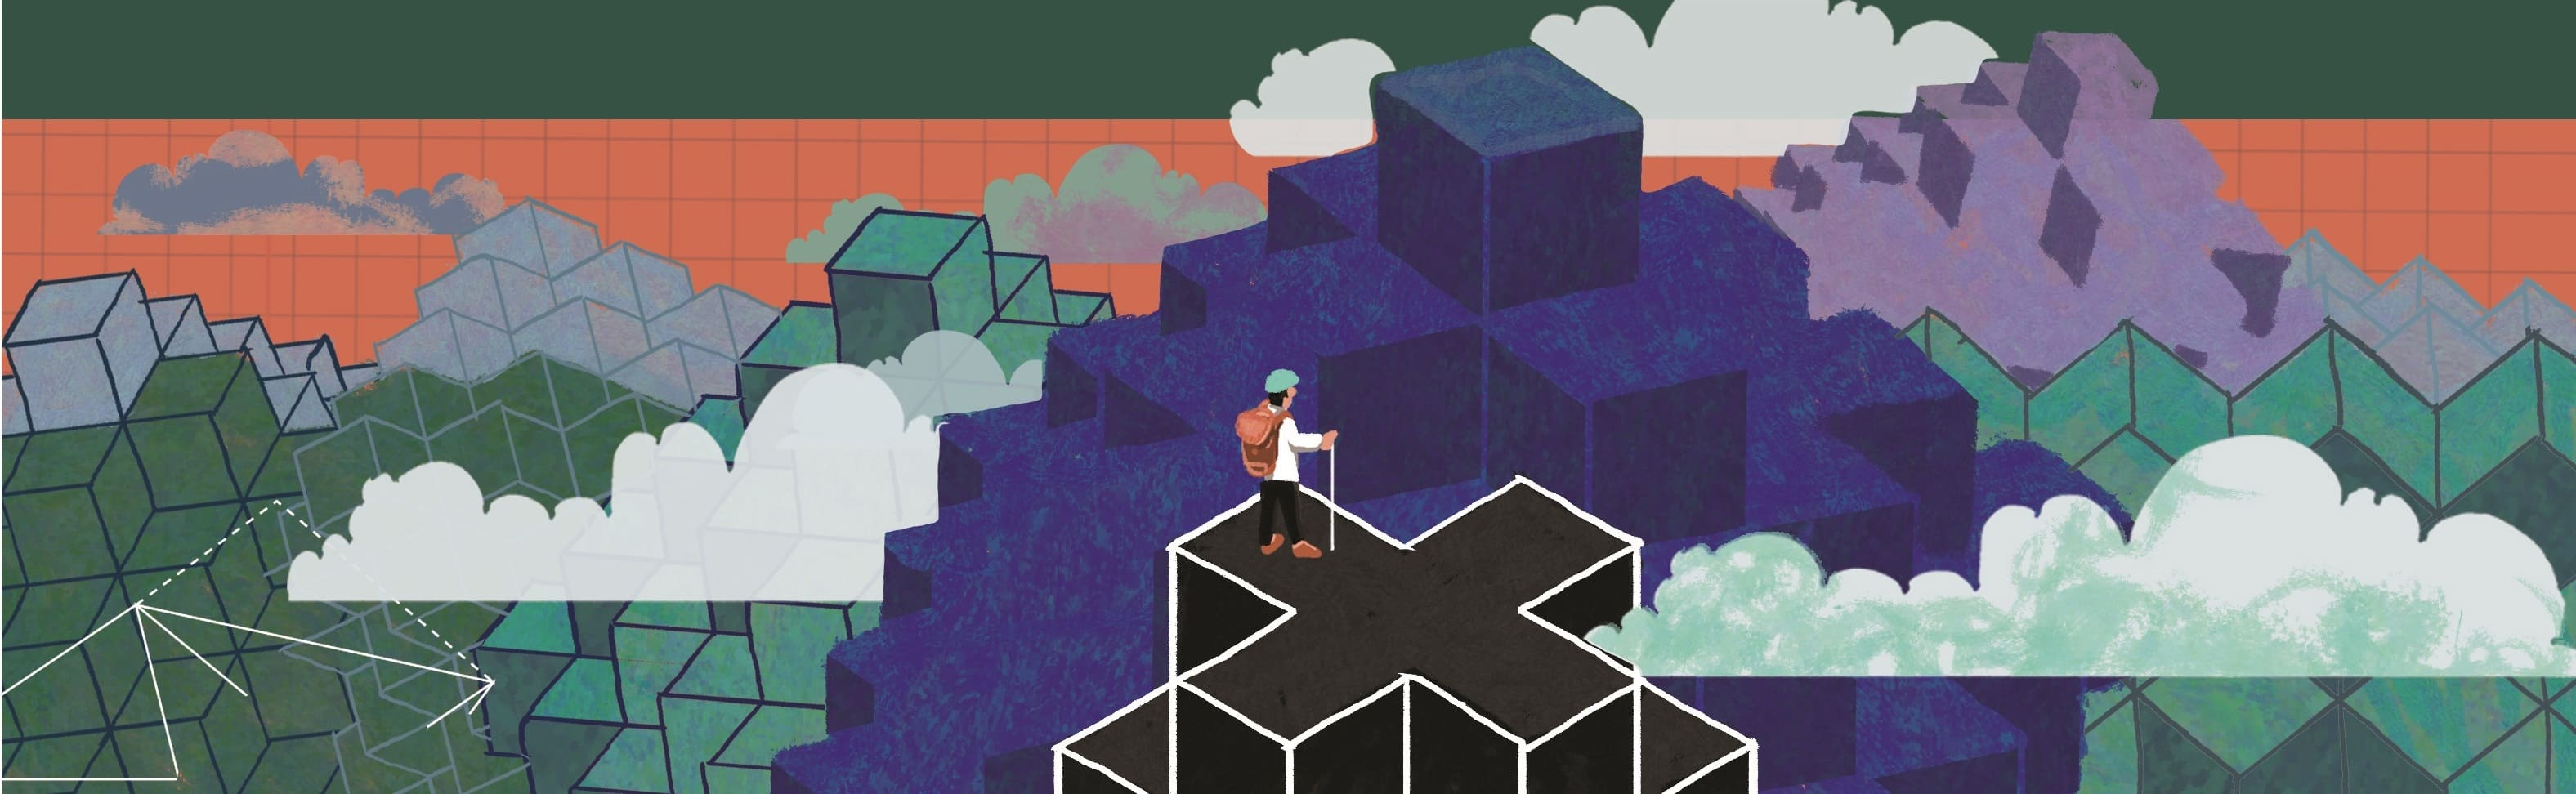
\includegraphics[width=19.3cm]{../thachthuctoanhoc/bannerthachthuc}}}
\centering
\vspace*{4cm}
\endgroup
\vspace*{-8pt}
\begin{tBox}
	\begin{itemize}[leftmargin = 13pt, itemsep = 1.0pt] 
				\item Mỗi bài toán đề xuất (kèm theo lời giải) cần được nêu rõ là bài sáng tác hay bài sưu tầm.
%		\item Mỗi bài toán đề xuất (kèm theo lời giải) cần được nêu rõ là bài sáng tác hay bài sưu tầm (nếu là bài sưu tầm, cần ghi rõ nguồn).
		\item Bài giải cho mỗi bài toán cần được trình bày trong một file riêng hoặc
		một tờ giấy riêng.
		\item  Người đề xuất bài toán hoặc gửi bài giải cho các bài toán trong mục ``Thách thức kỳ này" cần ghi rõ họ, đệm, tên và nơi làm việc/học tập, số điện thoại liên hệ. Nếu là học sinh (hoặc sinh viên) cần ghi rõ là học sinh lớp mấy (hoặc sinh viên năm thứ mấy).
		\item Các bài toán trong mục Thách thức kỳ này hướng tới các độc giả là học sinh phổ thông; được phân chia thành các mức độ $B$, $A$, và được sắp xếp theo độ khó tăng dần, theo đánh giá chủ quan của Ban biên tập. Các bài toán mức độ $B$ không đòi hỏi các kiến thức vượt quá chương trình môn Toán cấp THCS; các bài toán mức độ $A$ không đòi hỏi các kiến thức vượt quá chương trình môn Toán cấp THPT.
		\item Cách thức gửi bài toán đề xuất hoặc lời giải: gửi file thu được bằng cách scan, ảnh chụp (rõ nét) của bản viết tay, hoặc được soạn thảo bằng các phần mềm Latex, Word tới \url{bbt@pi.edu.vn} hoặc gửi qua đường bưu điện tới Tòa soạn (xem địa chỉ tại bìa $2$).
		\item Hạn gửi lời giải cho các bài toán P$641$--P$650$: trước ngày $15/11/2022$.
	\end{itemize}
\end{tBox}
\begin{center}
	\vspace*{-5pt}
	\textbf{\color{thachthuctoanhoc}\color{thachthuctoanhoc}THÁCH THỨC KỲ NÀY}
	\vspace*{-5pt}
\end{center}
\begin{multicols}{2}
	\setlength{\abovedisplayskip}{4pt}
	\setlength{\belowdisplayskip}{4pt}
	{\color{thachthuctoanhoc}{\usefont{T5}{qag}{b}{n} P641.}}
	(Mức $B$) Tại mỗi đỉnh của một đa giác lồi $18$ cạnh ở Hình dưới đây, người ta ghi một số, sao cho số được ghi ở mỗi đỉnh bằng tổng hai số được ghi ở hai đỉnh kề với nó.
	\begin{figure}[H]
		\vspace*{-5pt}
		\centering
		\captionsetup{labelformat= empty, justification=centering}
		\definecolor{ffvvqq}{rgb}{1,0.3333333333333333,0}
		\definecolor{qqqqffa}{rgb}{0,0,1}
		\definecolor{qqzzff}{rgb}{0,0.6,1}
		\begin{tikzpicture}[line cap=round,line join=round,>=triangle 45,x=1cm,y=1cm,scale=0.42]
			\draw (1.401115339869085,5.50644760016908136) node[anchor=north west] {$X$};
			\draw (1.4408759814898973,-0.7306378725360659) node[anchor=north west] {$Y$};
			\draw (-7.8444170535279,2.5008856260029945) node[anchor=north west] {$S$};
			\draw [color=qqzzff] (0.0915547437082469,-1.9784020259611625)--(1.3147607160299626,-0.9781184915188108);
			\draw [color=qqzzff] (1.3147607160299626,-0.9781184915188108)--(2.122081224105652,0.3802016464606015); 
			\draw [color=qqzzff] (2.122081224105652,0.3802016464606015)--(2.4161414998796458,1.932724932666551); 
			\draw [color=qqzzff] (2.4161414998796458,1.932724932666551)--(2.1614735342261406,3.4921941459791768);
			\draw [color=qqzzff] (2.1614735342261406,3.4921941459791768)--(1.38879404230183,4.87051428395859);
			\draw [color=qqzzff] (1.38879404230183,4.87051428395859)--(0.19129957436757605,5.901439596125702);
			\draw [color=qqzzff] (0.19129957436757605,5.901439596125702)--(-1.2865743636076452,6.4606252749959765);
			\draw [color=qqzzff] (-1.2865743636076452,6.4606252749959765)--(-2.866574363607645,6.480625274995977);
			\draw [color=qqzzff] (-2.866574363607645,6.480625274995977)--(-4.358129107315893,5.959027300957139);
			\draw [color=qqzzff] (-4.358129107315893,5.959027300957139)--(-5.581335079637608,4.958743766514788);
			\draw [color=qqzzff] (-5.581335079637608,4.958743766514788)--(-6.388655587713298,3.600423628535374);
			\draw [color=qqzzff] (-6.388655587713298,3.600423628535374)--(-6.682715863487291,2.0479003423294264);
			\draw [color=qqzzff] (-6.682715863487291,2.0479003423294264)--(-6.428047897833785,0.4884311290167975);
			\draw [color=qqzzff] (-6.428047897833785,0.4884311290167975)--(-5.655368405909476,-0.889889008962613);
			\draw [color=qqzzff] (-5.655368405909476,-0.889889008962613)--(-4.457873937975224,-1.9208143211297237);
			\draw [color=qqzzff] (-4.457873937975224,-1.9208143211297237)--(-2.98,-2.48);
			\draw [color=qqzzff] (-2.98,-2.48)--(-1.4,-2.5);
			\draw [color=qqzzff] (-1.4,-2.5)--(0.0915547437082469,-1.9784020259611625);
			\draw [fill=qqqqffa] (-2.98,-2.48) circle (1.6pt);
			\draw [fill=qqqqffa] (-1.4,-2.5) circle (1.6pt);
			\draw [fill=qqqqffa] (0.0915547437082469,-1.9784020259611625) circle (1.6pt);
			\draw [fill=qqqqffa] (1.3147607160299626,-0.9781184915188108) circle (1.6pt);
			\draw [fill=qqqqffa] (2.122081224105652,0.3802016464606015) circle (1.6pt);
			\draw [fill=qqqqffa] (2.4161414998796458,1.932724932666551) circle (1.6pt);
			\draw [fill=qqqqffa] (2.1614735342261406,3.4921941459791768) circle (1.6pt);
			\draw [fill=qqqqffa] (1.38879404230183,4.87051428395859) circle (1.6pt);
			\draw [fill=qqqqffa] (0.19129957436757605,5.901439596125702) circle (1.6pt);
			\draw [fill=qqqqffa] (-1.2865743636076452,6.4606252749959765) circle (1.6pt);
			\draw [fill=qqqqffa] (-2.866574363607645,6.480625274995977) circle (1.6pt);
			\draw [fill=qqqqffa] (-4.358129107315893,5.959027300957139) circle (1.6pt);
			\draw [fill=qqqqffa] (-5.581335079637608,4.958743766514788) circle (1.6pt);
			\draw [fill=qqqqffa] (-6.388655587713298,3.600423628535374) circle (1.6pt);
			\draw [fill=qqqqffa] (-6.682715863487291,2.0479003423294264) circle (1.6pt);
			\draw [fill=qqqqffa] (-6.428047897833785,0.4884311290167975) circle (1.6pt);
			\draw [fill=qqqqffa] (-5.655368405909476,-0.889889008962613) circle (1.6pt);
			\draw [fill=qqqqffa] (-4.457873937975224,-1.9208143211297237) circle (1.6pt);
		\end{tikzpicture}
		\vspace*{-5pt}
	\end{figure}
	Biết rằng, số được ghi ở đỉnh $X$ là $20$, và số được ghi ở đỉnh $Y$ là $22$. Hãy tìm số được ghi ở đỉnh $S$. 
	\vskip 0.05cm
	\hfill	\textit{Bùi Văn Biên, France (st)}
	\vskip 0.05cm
	{\color{thachthuctoanhoc}{\usefont{T5}{qag}{b}{n} P642.}}
	(Mức $B$) Cho $x,y$ là các số nguyên dương thoả mãn $y^2+x-1$ chia hết cho \linebreak $xy+1$. Chứng minh rằng, tồn tại số tự nhiên $z$ sao cho $x+y+z+xyz$ là số chính phương.
	\begin{flushright}
		\textit{Nguyễn Đức Tấn, Tp. Hồ Chí Minh}
	\end{flushright}
	{\color{thachthuctoanhoc}{\usefont{T5}{qag}{b}{n} P643.}}
	(Mức $B$) Người ta lần lượt ghi các số lên bảng, theo quy tắc: Ở mỗi lần ghi, chỉ ghi một số, và nếu số được ghi ở lần thứ $k$ ($k\in\mathbb N^*$) là $x\neq-1$, thì ở lần thứ $k+1$ ghi số $\dfrac{x-1}{x+1}$. Hãy tìm số nhỏ nhất cần ghi ở lần thứ nhất, sao cho trong quá trình ghi số lên bảng theo quy tắc trên, ta ghi được số $-\dfrac1{2023}$. 
	\begin{flushright}
		\textit{Phùng Chí Tự, Hà Nội}
	\end{flushright}
	{\color{thachthuctoanhoc}{\usefont{T5}{qag}{b}{n} P644.}}
	(Mức $B$) Xét tam giác $ABC$ có các góc $B,C$ nhọn. Gọi $H$ là chân đường cao kẻ từ $A$ của tam giác đó.  Chứng minh rằng, $ABC$ là tam giác vuông tại $A$ khi và chỉ khi 
	\begin{align*}
		\dfrac{HB^3}{AB^4}+\dfrac{HC^3}{AC^4}=\dfrac1{BC}\cdot
	\end{align*} 
	\begin{center} 
		\definecolor{ffqqqq}{rgb}{1,0,0}
		\definecolor{qqzzff}{rgb}{0,0.6,1}
		\definecolor{qqqqff}{rgb}{0,0,1}
		\definecolor{qqqqffa}{rgb}{1,1,1}
		\definecolor{cqcqcq}{rgb}{0.7529411764705882,0.7529411764705882,0.7529411764705882}
		\begin{tikzpicture}[line cap=round,line join=round,>=triangle 45,x=1cm,y=1cm, scale=0.6]
			\draw (-2.8771572875253812,-2) -- (-2.8771572875253812,-1.7171572875253809) -- (-3.16,-1.7171572875253809) -- (-3.16,-2) -- cycle; 
			\draw [color=qqzzff] (-3.16,4.66)-- (-5.54,-2);
			\draw [color=qqzzff] (-5.54,-2)-- (2,-2);
			\draw [color=qqzzff] (2,-2)-- (-3.16,4.66);
			\draw [,color=ffqqqq] (-3.16,4.66)-- (-3.16,-2);
			\draw [fill=qqqqffa] (-3.16,4.66) circle (1.6pt);
			\draw[color=qqqqff] (-3.18,5.11) node {$A$};
			\draw [fill=qqqqffa] (-5.54,-2) circle (1.6pt);
			\draw[color=qqqqff] (-5.7,-2.5) node {$B$};
			\draw [fill=qqqqffa] (2,-2) circle (1.6pt);
			\draw[color=qqqqff] (2,-2.5) node {$C$};
			\draw [fill=qqqqffa] (-3.16,-2) circle (1.6pt);
			\draw[color=qqqqff] (-3.18,-2.5) node {$H$};
		\end{tikzpicture}
	\end{center}
	\begin{flushright}
		\textit{Trần Quang Hùng, Hà Nội}
	\end{flushright}
	{\color{thachthuctoanhoc}{\usefont{T5}{qag}{b}{n} P645.}}
	(Mức $B$) Cho $a,b,c$ là các số thực dương thoả mãn $abc=1$. Chứng minh rằng 
	\begin{align*}
		\dfrac{a}{a\!+\!b^{3} c\!+\!b}+\dfrac{b}{b\!+\!c^{3} a\!+\!c}+\dfrac{c}{c\!+\!a^{3} b\!+a} \ge 1.
	\end{align*}
	\begin{flushright}
		\textit{Đào Văn Nam, Hà Nội}
	\end{flushright}
	{\color{thachthuctoanhoc}{\usefont{T5}{qag}{b}{n} P646.}}
	(Mức $B$) Chứng minh rằng, trong mỗi bát giác lồi, luôn có ít nhất ba đường chéo, mà độ dài của chúng đôi một khác nhau. 
	\vskip 0.05cm
	(Bát giác là một đa giác có $8$ cạnh.)
	\begin{flushright}
		\textit{Phạm Nhật Nguyệt, Hải Phòng}
	\end{flushright}
	{\color{thachthuctoanhoc}{\usefont{T5}{qag}{b}{n} P647.}}
	(Mức $A$) Cho số nguyên $n\ge2$, và cho $n$ điểm phân biệt $A_1,\ldots,A_n$ cùng nằm trên một đường tròn, theo chiều kim đồng hồ. Một dãy điểm  $A_{k_1},\ldots,A_{k_t}$, gồm ít nhất hai điểm  (trong $n$ điểm đó), không có hai điểm nào trùng nhau, được gọi là một {\it đường đi}, nếu đường gấp khúc $A_{k_1}\ldots A_{k_t}$ (gồm $t-1$ đoạn thẳng) không tự cắt.  Hỏi, có tất cả bao nhiêu đường đi?
	\begin{flushright}
		\textit{Nguyễn Tường Thanh, Nghệ An (st)}
	\end{flushright}
	{\color{thachthuctoanhoc}{\usefont{T5}{qag}{b}{n} P648.}}
	(Mức $A$) Xét số thực $a$ và xét tất cả các hàm số $f: \mathbb R \rightarrow \mathbb R,$ thỏa mãn
	\begin{align*}
		f(a x+y+f(x+y))+f(x y)=y f(x)
	\end{align*}
	với mọi $x,y\in\mathbb R$. 
	\vskip 0.05cm
	$a)$ Tìm tất cả các số thực $a$, sao cho trong các hàm số $f$, tồn tại một hàm là đơn ánh từ $\mathbb R$ đến $\mathbb R$. 
	\vskip 0.05cm
	$b)$ Khi $a=2$, tìm tất cả các hàm số $f$ có $f(0)=0$. 
	\begin{flushright}
		\textit{Lê Phúc Lữ, Tp. Hồ Chí Minh}
	\end{flushright}
	{\color{thachthuctoanhoc}{\usefont{T5}{qag}{b}{n} P649.}}
	(Mức $A$) Cho tam giác $A B C$ và điểm $D$ cố định nằm trên $B C$ ($D$ khác $B,C$). Một đường tròn $(O)$ thay đổi,  đi qua $B, C$ và cắt các cạnh $A B, A C$ tương ứng tại $E, F$. Gọi $G$ là giao điểm của $B F$ và $A D$. Chứng minh rằng, đường thẳng $G E$ luôn đi qua một điểm cố định.
	\begin{center}
		\definecolor{ffqqqq}{rgb}{1,0,0}
		\definecolor{qqzzff}{rgb}{0,0.6,1}
		\definecolor{qqqqff}{rgb}{0,0,1}
		\definecolor{qqqqffa}{rgb}{1,1,1}
		\begin{tikzpicture}[line cap=round,line join=round,>=triangle 45,x=1cm,y=1cm,scale=0.6]
			\draw [color=qqzzff] (-4.81309,-1)-- (-2.9915435035522586,4.9363824736365585);
			\draw [color=qqzzff] (-2.9915435035522586,4.9363824736365585)-- (2.16949,-1);
			\draw [color=qqzzff] (2.16949,-1)-- (-4.81309,-1);
			\draw [thachthuctoanhoc] (-1.3218,-0.16393583791880353) circle (3.590001273985364cm);
			\draw [] (-4.81309,-1)-- (-1.6642556805547637,3.409694424723417);
			\draw [] (-2.9915435035522586,4.9363824736365585)-- (-0.3604269142578283,-1);
			\draw [,color=ffqqqq] (-6.227177601372653,1.9518434021508382)-- (2.997592242483252,3.9372366050655776);
			\draw [fill=qqqqffa] (-2.9915435035522586,4.9363824736365585) circle (1.6pt);
			\draw[color=qqqqff] (-3.0725009370690106,5.432246753926664) node {$A$};
			\draw [fill=qqqqffa] (-4.81309,-1) circle (1.6pt);
			\draw[color=qqqqff] (-5.177394208504555,-1.1455447193094175) node {$B$};
			\draw [fill=qqqqffa] (2.16949,-1) circle (1.6pt);
			\draw[color=qqqqff] (2.531407750174166,-1.2062627944469815) node {$C$};
			\draw [fill=qqqqffa] (-1.3218,-0.16393583791880353) circle (1.6pt);
			\draw[color=qqqqff] (-1.721554748380367,-0.3966884592794637) node {$O$};
			\draw [fill=qqqqffa] (-3.7432966215398427,2.4864345624380344) circle (1.6pt);
			\draw[color=qqqqff] (-4.064229497649219,2.801130164632231) node {$E$};
			\draw [fill=qqqqffa] (-1.6642556805547637,3.409694424723417) circle (1.6pt);
			\draw[color=qqqqff] (-1.5545490586299158,3.873816158729192) node {$F$};
			\draw [fill=qqqqffa] (-0.3604269142578283,-1) circle (1.6pt);
			\draw[color=qqqqff] (-0.36042691425782825,-1.507459586342921) node {$D$};
			\draw [fill=qqqqffa] (-2.0657079453674543,2.847492151010585) circle (1.6pt);
			\draw[color=qqqqff] (-2.161729810005554,2.11658235542766) node {$G$};
		\end{tikzpicture}
	\end{center}
	\begin{flushright}
		\textit{Phạm Vĩnh Minh, Đồng Tháp}
	\end{flushright}
	{\color{thachthuctoanhoc}{\usefont{T5}{qag}{b}{n} P650.}}
	(Mức $A$) Cho $p$ là một số nguyên tố có dạng $4k+3$, $k\in\mathbb N$.  Xét dãy số Fibonacci $(F_n)$, xác định bởi: $F_0=0$, $F_1=1$, và 
	\begin{align*}
		F_{n+2}=F_{n+1}+F_n\quad\text{\color{black}với mọi } n\ge0.
	\end{align*}
	Chứng minh rằng, không tồn tại các số nguyên dương $m,\,n$, với $n\ge 5$, sao cho \linebreak$F_n=p^m$.
	\begin{flushright}
		\textit{Nguyễn Song Minh, Hà Nội (st)}
	\end{flushright}
\end{multicols}
\begin{center}
	{\large{\textbf{\color{thachthuctoanhoc}GIẢI BÀI KỲ TRƯỚC}}}
\end{center}
\begin{multicols}{2}
	\setlength{\abovedisplayskip}{4pt}
	\setlength{\belowdisplayskip}{4pt}
	{\color{thachthuctoanhoc}{\usefont{T5}{qag}{b}{n} P611.}}
	(Mức $B$) Cho $A,B,C$ là các chữ số khác $0$ sao cho $\overline{CCA}+\overline{B2B}=\overline{A88}$. Hãy tìm số $\overline{ABC}$.
	\vskip 0.05cm
	\textbf{Lời giải} (\textit{dựa theo lời giải của bạn Phùng Việt Cường, lớp $10$T$2$, trường THPT chuyên Lê Hồng Phong, tỉnh Nam Định})\textbf{.}
	\vskip 0.05cm
	Viết lại giả thiết của bài ra dưới dạng:
	\begin{align*}
		\begin{array}{l}
			\underline \begin{array}{l}
				\overline {CCA} \\
				\overline {B2B} 
			\end{array} \\
			\overline {A88} 
		\end{array}
	\end{align*}
	Theo quy tắc ``cộng dọc", từ phép cộng ở hàng trăm, suy ra
	\begin{align*}
		C + B \le A \le 9.
	\end{align*}
	Do đó, $B < 9$ (vì $C > 0$); suy ra, $A + B < 18$. Vì thế, từ phép cộng ở hàng đơn vị, ta được
	\begin{align*}
		A + B = 8. \tag{$1$}
	\end{align*}                                                                  
	Do đó, từ phép cộng ở hàng chục, với lưu ý $C + 2 \le 11$, ta có $C + 2 = 8$. Vì thế, $C = 6$. Do đó, từ phép cộng ở hàng trăm, ta có
	\begin{align*}
		6 + B = A, \text{\color{black} hay }A - B = 6. \tag{$2$}
	\end{align*}
	Từ ($1$) và ($2$), ta được $A = 7$ và $B = 1$.
	\vskip 0.05cm
	Vậy, $\overline {ABC} \,\, = \,\,716$.
	\vskip 0.05cm
	\textbf{Bình luận và Nhận xét}
	\vskip 0.05cm
	Rất tiếc, trong số các lời giải Tạp chí đã nhận được từ bạn đọc, có ba lời giải không đúng, do người giải bài đã mắc một trong các lỗi sau:
	\vskip 0.05cm
	$\bullet$  Với $a$, $b$, $c$, $x$, $y$, $z$, $u$, $v$, $t$ là các số nguyên, từ
	\begin{align*}
		ax + by + cz = au + bv + ct,
	\end{align*}
	suy ra, $x = u$, $y = v$ và $z = t$.
	\vskip 0.05cm
	$\bullet$  Khi xét phép cộng ở hàng chục của phép ``cộng dọc", quên trường hợp ``có nhớ từ phép cộng ở hàng đơn vị".
	\begin{flushright}
		\textbf{Lê Huy}
	\end{flushright}
	{\color{thachthuctoanhoc}{\usefont{T5}{qag}{b}{n} P612.}}
	(Mức $B$) Chứng minh biểu thức sau nhận giá trị nguyên, với mọi giá trị nguyên dương của $n$:
	\begin{align*}
		A\!=\!\dfrac{\left(2^4\!+\!\dfrac14\right)\!\left(4^4\!+\!\dfrac14\right)\!\cdots\! \left((2n)^4\!+\!\dfrac14\right)}{\left(1^4\!+\!\dfrac14\right)\left(3^4\!+\!\dfrac14\right)\!\cdots\! \left((2n\!-\!1)^4\!+\!\dfrac14\right)}.
	\end{align*}
	\textbf{Lời giải} (\textit{dựa theo tuyệt đại đa số lời giải Tạp chí đã nhận được từ bạn đọc})\textbf{.}
	\vskip 0.05cm
	Với mọi số nguyên dương $m$, ta có:
	\begin{align*}
		{m^4}\, + \,\,\frac{1}{4}\,\, = \,\,{m^4}\, + \,\,2 \cdot {m^2} \cdot \frac{1}{2}\,\, + \,\,\frac{1}{4}\,\, - \,\,{m^2}\, = \,\,{\left( {{m^2}\, + \,\,\frac{1}{2}} \right)^2}\, - \,\,{m^2}\\
		\,\,\,\,\,\,\,\,\,\,\,\,\,\,\,\, = \,\,\left( {{m^2}\, - \,\,m\,\, + \,\,\frac{1}{2}} \right)\left( {{m^2}\, + \,\,m\,\, + \,\,\frac{1}{2}} \right).
	\end{align*}
	Do đó, với mọi số nguyên dương $k$, ta có:
	\begin{align*}
		{\left( {2k} \right)^4}\, + \,\,\frac{1}{4}\,\, = \,\,\left( {{{\left( {2k} \right)}^2}\, - \,\,2k\,\, + \,\,\frac{1}{2}} \right)\left( {{{\left( {2k} \right)}^2}\, + \,\,2k\,\, + \,\,\frac{1}{2}} \right);
	\end{align*}
	\begin{align*}
			{\left( {2k\,\, - \,\,1} \right)^4}\, + \,\,\frac{1}{4}\,\, = \,\,\left( {{{\left( {2k\,\, - \,\,1} \right)}^2}\, - \,\,\left( {2k\,\, - \,\,1} \right)\,\, + \,\,\frac{1}{2}} \right)\left( {{{\left( {2k\,\, - \,\,1} \right)}^2}\, + \,\,\left( {2k\,\, - \,\,1} \right)\,\, + \,\,\frac{1}{2}} \right)\\
			\,\,\,\,\,\,\,\,\,\,\,\,\,\,\,\,\,\,\,\,\,\,\,\,\,\,\,\,\,\, = \,\,\left( {{{\left( {2\left( {k\,\, - \,\,1} \right)} \right)}^2}\, + \,\,2\left( {k\,\, - \,\,1} \right)\,\, + \,\,\frac{1}{2}} \right)\left( {{{\left( {2k} \right)}^2}\, - \,\,2k\,\, + \,\,\frac{1}{2}} \right).
	\end{align*}
	Suy ra
	\begin{align*}
		\frac{{{{\left( {2k} \right)}^4}\, + \,\,\frac{1}{4}}}{{{{\left( {2k\,\, - \,\,1} \right)}^4}\, + \,\,\frac{1}{4}}}\,\, = \,\,\frac{{{{\left( {2k} \right)}^2}\, + \,\,2k\,\, + \,\,\frac{1}{2}}}{{{{\left( {2\left( {k\,\, - \,\,1} \right)} \right)}^2}\, + \,\,2\left( {k\,\, - \,\,1} \right)\,\, + \,\,\frac{1}{2}}}
	\end{align*}
	với mọi số nguyên dương $k$.
	\vskip 0.05cm
	Do đó
	
	Vì vậy, biểu thức A nhận giá trị nguyên tại mọi giá trị nguyên dương của n.
	Bình luận và Nhận xét
	Tất cả các lời giải Tạp chí nhận được từ bạn đọc đều là lời giải đúng.
	Hà Thanh
	P613. (Mức B) Cho n là một số nguyên dương. Chứng minh rằng, trong ba số n,   và  , có ít nhất hai số không phải là số chính phương.
	Lời giải (phỏng theo cách giải của bạn Trần Việt Anh, lớp 8C1, trường TH, THCS&THPT Archimedes, Đông Anh, Tp. Hà Nội).
	Trước hết, dễ dàng chứng minh được Nhận xét sau:
	Nhận xét 1: Với mọi số nguyên dương a, số dư trong phép chia   cho 5 chỉ có thể là 0, 1, hoặc 4.
	Từ đó, ta có:
	Nhận xét 2:   là số không chính phương.
	Chứng minh. Giả sử ngược lại,   là số chính phương.
	Khi đó, tồn tại số nguyên dương m, sao cho
	hay                                                  (1)
	Từ Nhận xét 1 suy ra, số dư trong phép chia   cho 5 sẽ là 4, 1, hoặc 2. Điều này mâu thuẫn với (1), do 15n chia hết cho 5. Mâu thuẫn nhận được cho thấy giả sử ở trên là sai; vì thế, Nhận xét 2 được chứng minh.
	Tiếp theo, giả sử n và   cùng là số chính phương. Khi đó, tồn tại các số nguyên dương x, y, sao cho   và   hay   Từ đây, ta có:
	;                                                                 (2)
	suy ra,                                                                                                                         (3)
	Theo Nhận xét 1,   và  
	Vì thế, từ (3) suy ra
	
	Do đó,   suy ra,   (do 5 là số nguyên tố). Vì thế
	
	do đó, từ (2) suy ra,   là điều vô lí. Điều vô lí này cho thấy, trong hai số n và   chỉ có tối đa một số là số chính phương. Từ đây và Nhận xét 2, hiển nhiên ta có điều phải chứng minh theo yêu cầu đề bài.
	Bình luận và Nhận xét
	Rất tiếc, trong số các lời giải Tạp chí đã nhận được từ bạn đọc, có một lời giải sai, do người giải bài đã ngộ nhận rằng, ``cả ba số đồng thời là số chính phương" là khẳng định ngược lại với khẳng định cần chứng minh theo yêu cầu đề bài.
	Lưu Thị Thanh Hà
	P614. (Mức B) Cho a, b là các số nguyên dương, thỏa mãn
	
	Chứng minh rằng, 4b + 1 là một số chính phương.
	(Với x là một số thực, {x} = x - [x], trong đó, [x] là số nguyên lớn nhất không vượt quá x. {x} được gọi là phần lẻ của số thực x.)
	Lời giải (dựa theo cách giải của bạn Nguyễn Đức Khải, lớp 10T2, trường THPT chuyên Lê Hồng Phong, tỉnh Nam Định).
	Viết lại hệ thức của đề bài dưới dạng:
	
	Từ đó, suy ra
	
	Vì thế, đặt   ta có   và
	;
	suy ra
	(1)
	Do đó
	
	Vì thế, đặt   ta có   và
	
	Do đó
	(2)
	Suy ra,   (do  ).                                                                                                   (3)
	Vì   nên hoặc   hoặc   là số vô tỉ.
	Nếu   thì từ (1) suy ra,   (do  ) và   là số chính phương, là điều vô lí, do
	
	Vì vậy,   là số vô tỉ. Kết hợp với (3) suy ra, x = 0 hoặc y = 0.
	Nếu y = 0 thì   (suy ra từ định nghĩa của y) và đồng thời,   (theo (2)). Do đó
	;
	suy ra
	
	là điều vô lí, do  
	Do đó, x = 0. Vì thế, từ định nghĩa của y và (2), suy ra
	
	Do đó
	
	là một số chính phương.
	Ta có điều phải chứng minh theo yêu cầu đề bài.
	Bình luận và Nhận xét
	
	Lưu Thị Thanh Hà
	P615. (Mức B) Cho tam giác ABC vuông tại A. Một điểm D di chuyển trên tia CA. Gọi E là hình chiếu vuông góc của C trên đường thẳng BD; F là giao điểm của AE và BC. Chứng minh rằng, đường thẳng DF luôn đi qua một điểm cố định.
	Lời giải ().
	
	Bình luận và Nhận xét
	
	Hạ Vũ Anh
	P616. (Mức B) Xét các số dương a, b, c thỏa mãn a + b + c = 4. Tìm giá trị nhỏ nhất của biểu thức
	
	Lời giải (dựa theo lời giải của bạn Trần Việt Anh, lớp 8C1, trường TH, THCS&THPT Archimedes, Đông Anh, Tp. Hà Nội).
	Do a, b, c có vai trò như nhau trong biểu thức P nên không mất tính tổng quát, có thể giả sử a = max{a, b, c}.
	Xét hai trường hợp sau:
	• Trường hợp 1: a > 2.
	Khi đó,   suy ra
	
	Do đó
	
	Vì thế
	
	• Trường hợp 2: 0 < a \le 2.
	Khi đó,   do đó, với lưu ý tới các giả thiết của bài ra, ta có:
	
	Như vậy, với mọi số thực dương a, b, c, thỏa mãn điều kiện của đề bài, ta luôn có  .
	Hơn nữa, với a = 2, b = c = 1, ta có a, b, c > 0, a + b + c = 4, và  .
	Vì vậy, giá trị nhỏ nhất của P bằng  .
	Bình luận và Nhận xét
	1. Ở lời giải trên, ta đã sử dụng (không chứng minh) bất đẳng thức ``trị tuyệt đối" rất cơ bản sau:
	``Cho số nguyên n  2. Khi đó, với mọi  , ta có:
	"
	Bạn đọc có thể dễ dàng chứng minh bất đẳng thức trên bằng phương pháp quy nạp theo n  2.
	2. Rất tiếc, có tới một nửa số lời giải Tạp chí nhận được từ bạn đọc là lời giải sai, hoặc không hoàn chỉnh, do người giải bài đã mắc một trong các lỗi sau:
	♦ Ngộ nhận rằng, với  , nếu x  y thì  
	♦ Khẳng định giá trị nhỏ nhất của P bằng  , ngay sau khi mới chỉ chứng minh được  .
	Nguyễn Khắc Minh
	P617. (Mức A) Giải phương trình
	
	Lời giải (dựa theo lời giải của bạn Trần Hữu Dương, lớp 10 Toán 1, trường THPT chuyên Hưng Yên, tỉnh Hưng Yên).
	Điều kiện xác định của phương trình:                                                                                        (1)
	Đặt    ; khi đó, phương trình đã cho được viết lại dưới dạng:
	(2)
	Từ định nghĩa của a, b, ta có:
	(3)
	(4)
	Từ (2) và (3), suy ra
	(5)
	Do (1), và do a  0, b > 0, nên a + x > 0, x + b > 0, và
	
	Vì thế, với lưu ý tới (3), (4), ta có:
	(5)   
	  
	  
	     
	    (do  ).
	Bằng cách thử trực tiếp, ta thấy x = 2 nghiệm đúng phương trình đã cho.
	Vậy, phương trình đã cho có nghiệm duy nhất x = 2.
	Bình luận và Nhận xét
	1. Ở lời giải trên, phép thử lại là bắt buộc, do phép biến đổi từ (2) sang (5) là phép biến đổi hệ quả.
	2. 
	Nguyễn Khắc Minh
	P618. (Mức A) Cho a, b, c là các số nguyên lớn hơn 1. Giả sử x, y, z là các số thực thỏa mãn     và   Tính giá trị của biểu thức
	T = x + y + z - xyz.
	Lời giải (dựa theo lời giải của các bạn: Nguyễn Đức Khải, Trần Đình Nam (lớp 10T2, trường THPT chuyên Lê Hồng Phong, tỉnh Nam Định) và Nguyễn Đình Khải Nguyên, Trần Thị Thanh Thư (lớp 11T2, 12T1, trường THPT chuyên Quốc học Huế, tỉnh Thừa Thiên - Huế)).
	Từ các giả thiết của bài ra, ta có:
	
	Từ đó, do a  1, suy ra
	xyz = x + y + z + 2.
	Vì thế
	T = x + y + z - xyz = 2.
	Bình luận và Nhận xét
	Tất cả các lời giải Tạp chí nhận được từ bạn đọc đều là lời giải đúng.
	Lê Huy
	P619. (Mức A) Cho tam giác ABC nội tiếp đường tròn (O), có trực tâm H. Gọi M là điểm chính giữa cung BAC của (O). Qua O, kẻ đường thẳng song song với AM, cắt HM tại P. Gọi X, Y, Z tương ứng là hình chiếu vuông góc của P trên BC, CA, AB. Chứng minh rằng, đường tròn ngoại tiếp tam giác XYZ đi qua trung điểm của HM.
	Lời giải ().
	
	Bình luận và Nhận xét
	
	Hạ Vũ Anh
	P620. (Mức A) Chứng minh rằng, với mọi số nguyên tố p  5, tồn tại số nguyên t, sao cho với mọi số nguyên k,   không chia hết cho p.
	Lời giải ().
	
	Bình luận và Nhận xét
	
	
	Hà Duy Hưng
	
\end{multicols}